% layouts
% EBS choices
% Geologies


\begin{frame}[ctb!]
  \frametitle{Clay Disposal Environments}

  \begin{figure}[h!]
    \begin{center}
      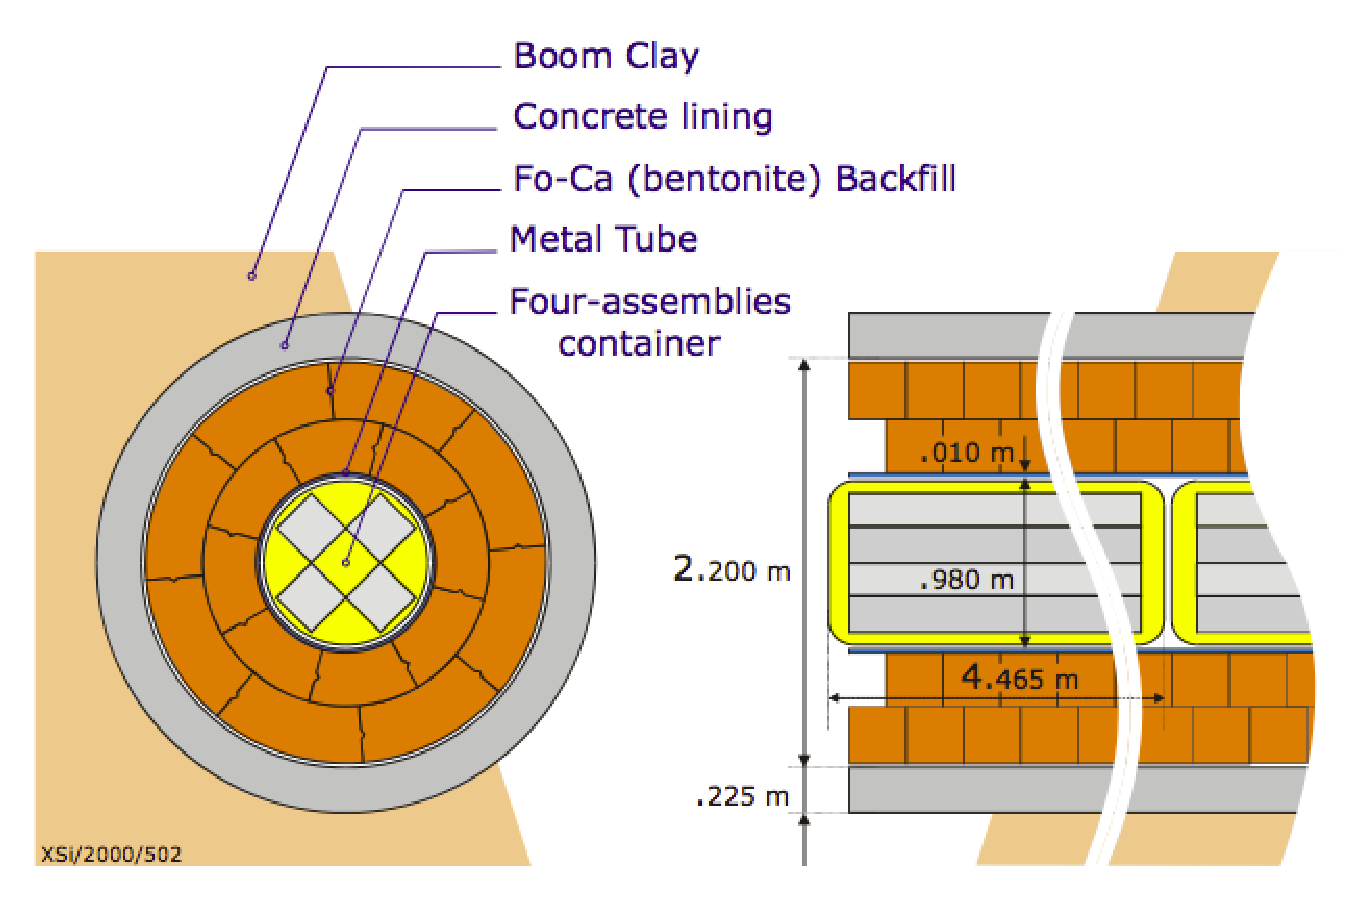
\includegraphics[height=.7\textheight]{belgianClayRedImp.eps}
    \end{center}
    \caption{Belgian reference concept in Boom Clay.\cite{von_lensa_red-impact_2005}}
    \label{fig:belgianClayRedImp}
  \end{figure}

\end{frame}

\begin{frame}[ctb!]
  \frametitle{Granite Disposal Environments}

  \begin{figure}[h!]
    \begin{center}
      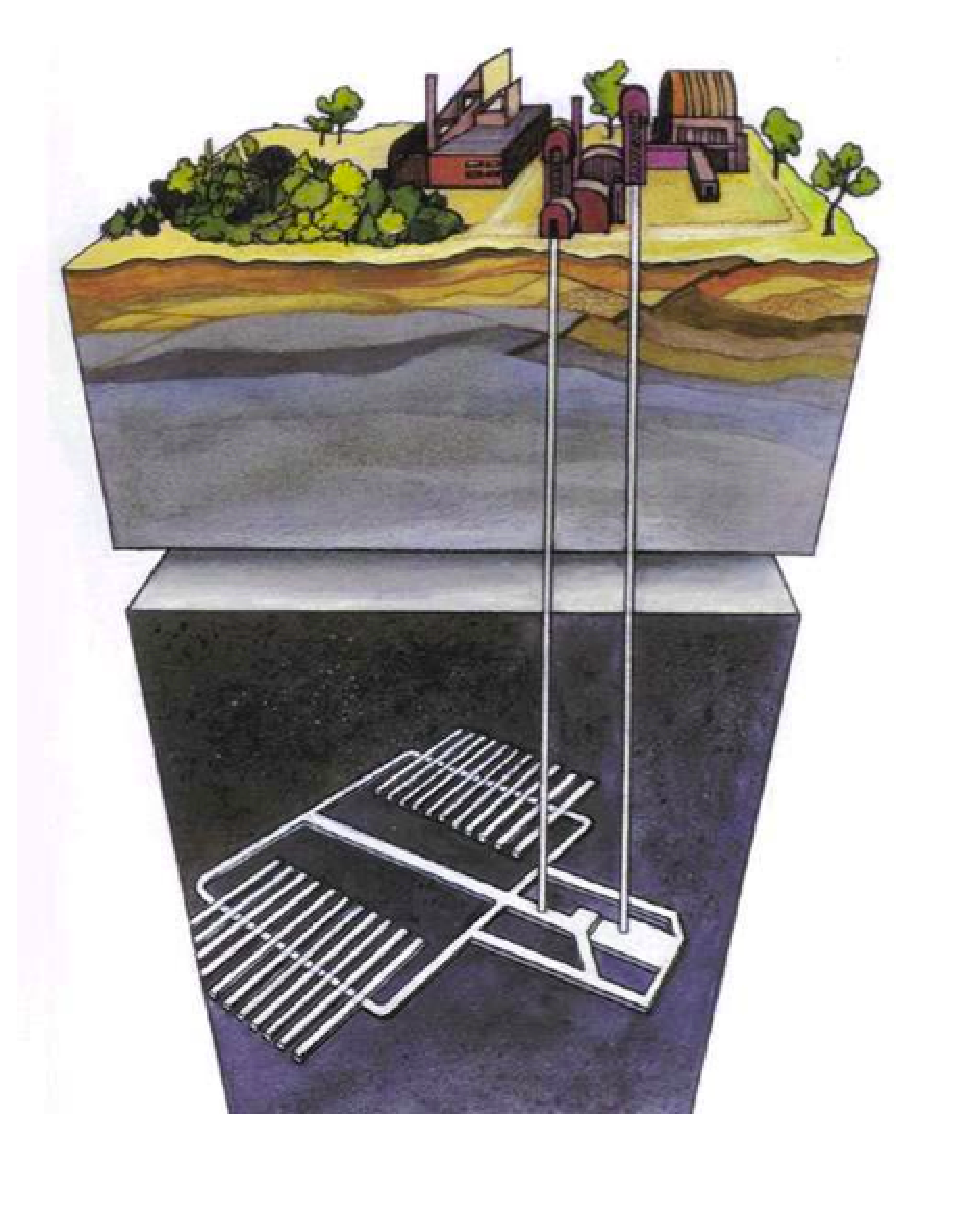
\includegraphics[height=.7\textheight]{czechGraniteRedImp.eps}
    \end{center}
    \caption{Czech reference concept in Granite.\cite{von_lensa_red-impact_2005}}
    \label{fig:czechGraniteRedImp}
  \end{figure}
\end{frame}

\begin{frame}[ctb!]
  \frametitle{Salt Disposal Environments}

  \begin{figure}[h!]
    \begin{center}
      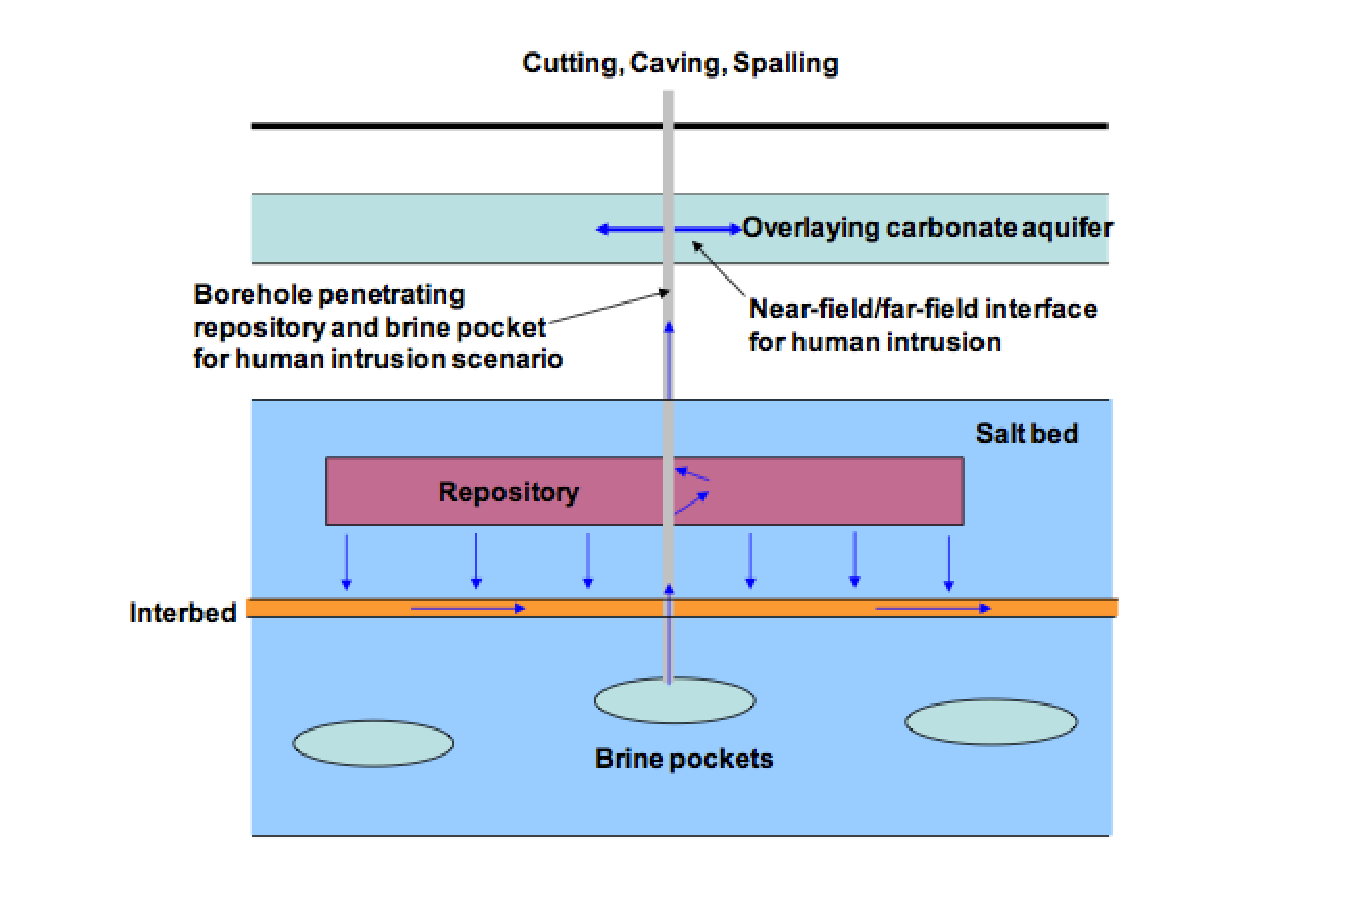
\includegraphics[height=.7\textheight]{saltGPAM.eps}
    \end{center}
    \caption{Used Fuel Division reference concept in Salt.\cite{clayton_generic_2010}}
    \label{fig:saltGPAM}
  \end{figure}
\end{frame}

\begin{frame}[ctb!]
  \frametitle{Deep Borehole Disposal Environment}

  \begin{figure}[h!]
    \begin{center}
      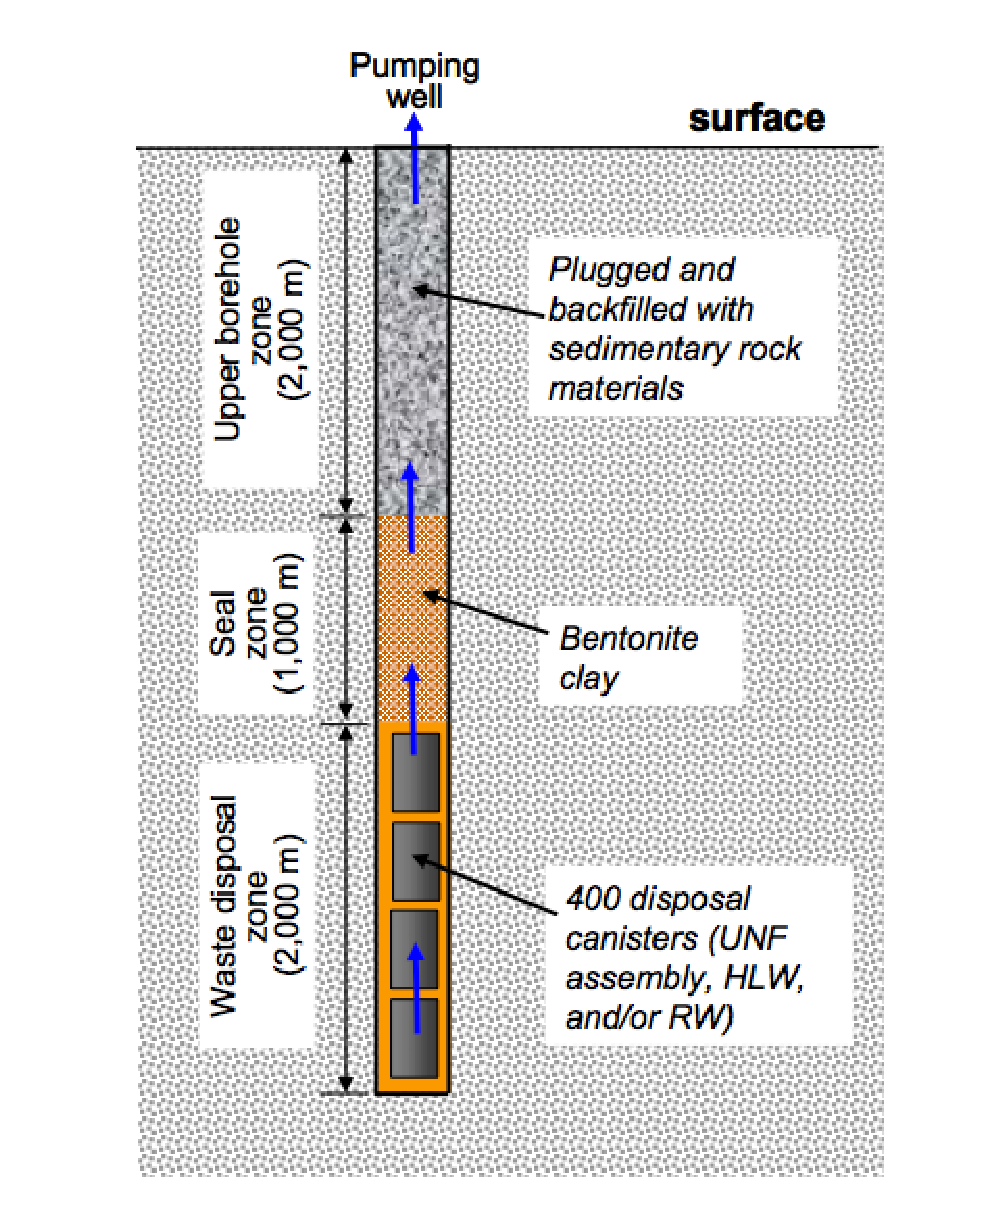
\includegraphics[height=.7\textheight]{boreholeGPAM.eps}
    \end{center}
    \caption{Used Fuel Division reference Deep Borehole concept.\cite{clayton_generic_2010}}
    \label{fig:boreholeGPAM}
  \end{figure}
\end{frame}


\begin{frame}
  \frametitle{Repository Layouts}
  \begin{minipage}{0.49\textwidth}
    \begin{figure}[h!]
      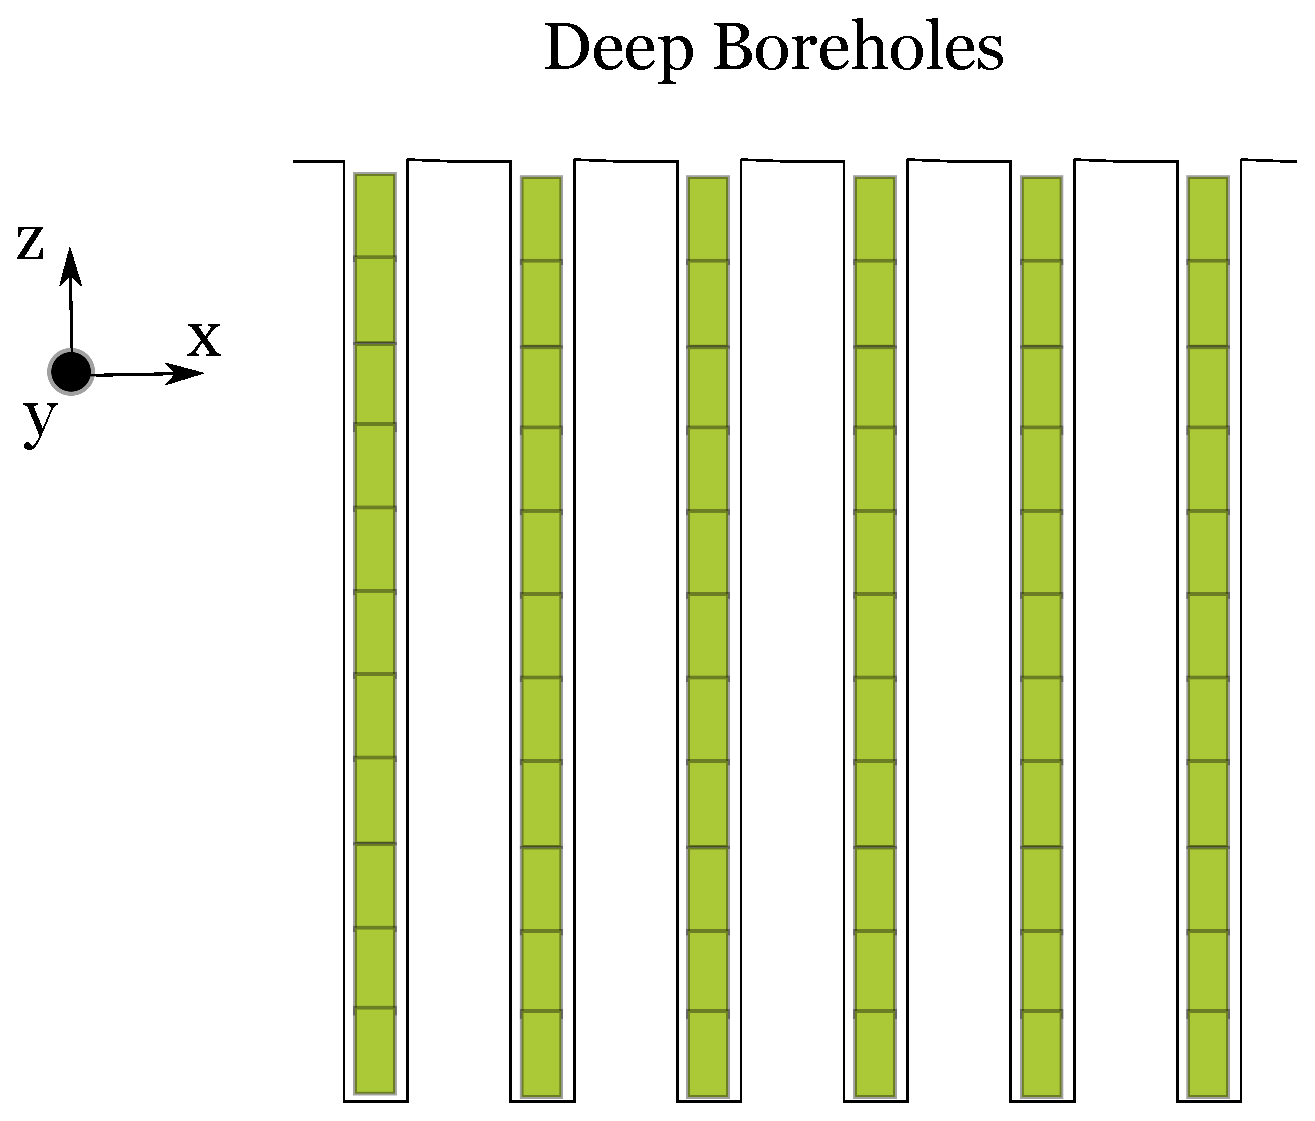
\includegraphics[width=0.75\textwidth]{boreholes.eps}
    \end{figure}
    \begin{figure}[h!]
      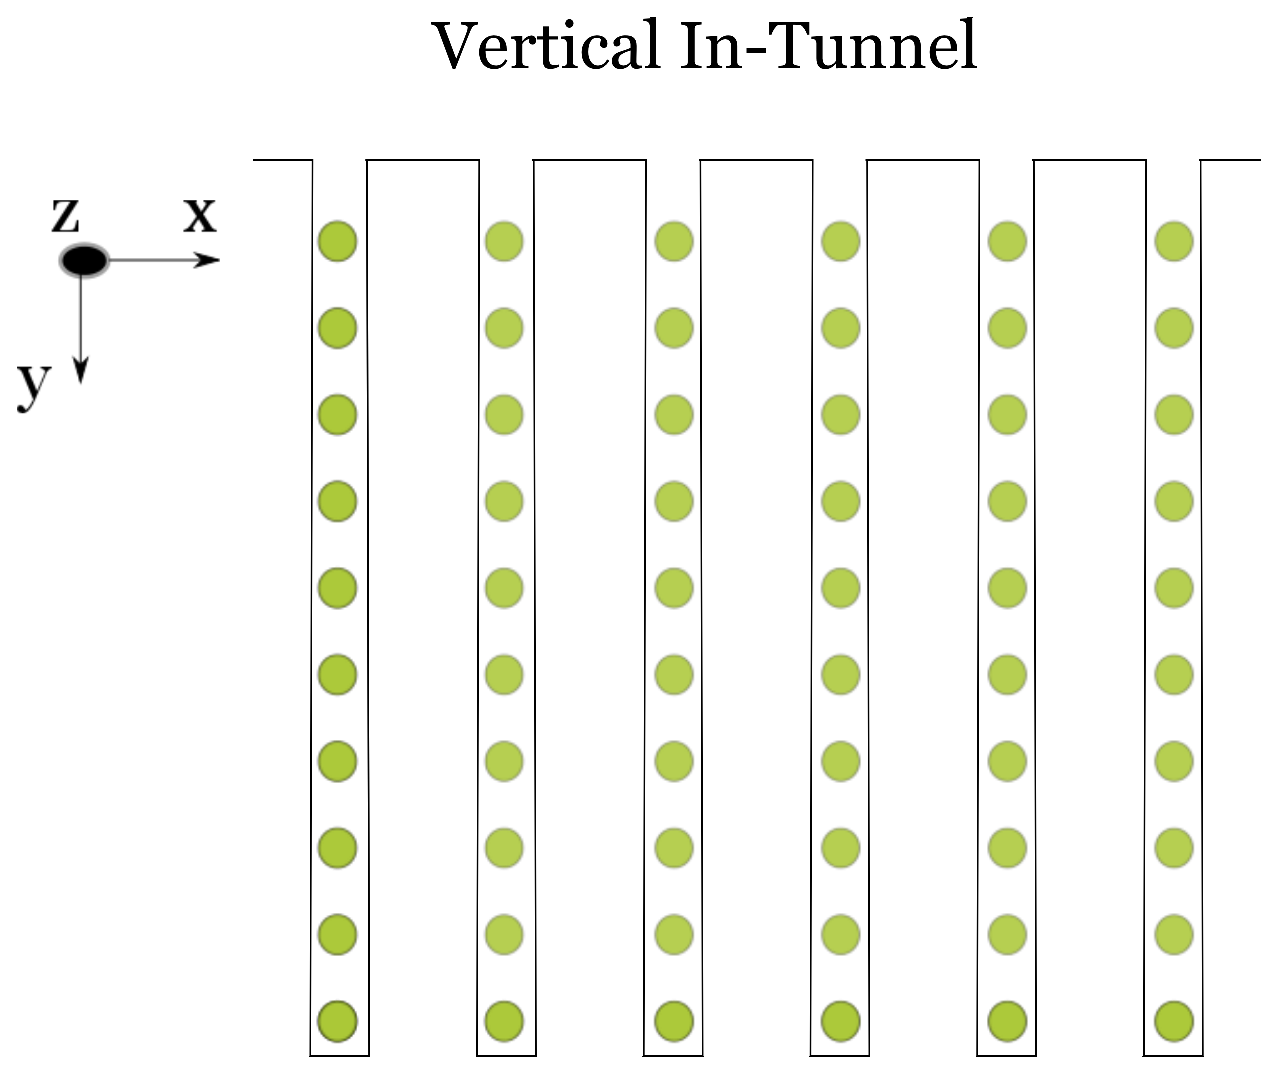
\includegraphics[width=0.75\textwidth]{vertical.eps}
    \end{figure}
  \end{minipage}
  \hspace{0.01cm}
  \begin{minipage}{0.49\textwidth}
    \begin{figure}[h!]
      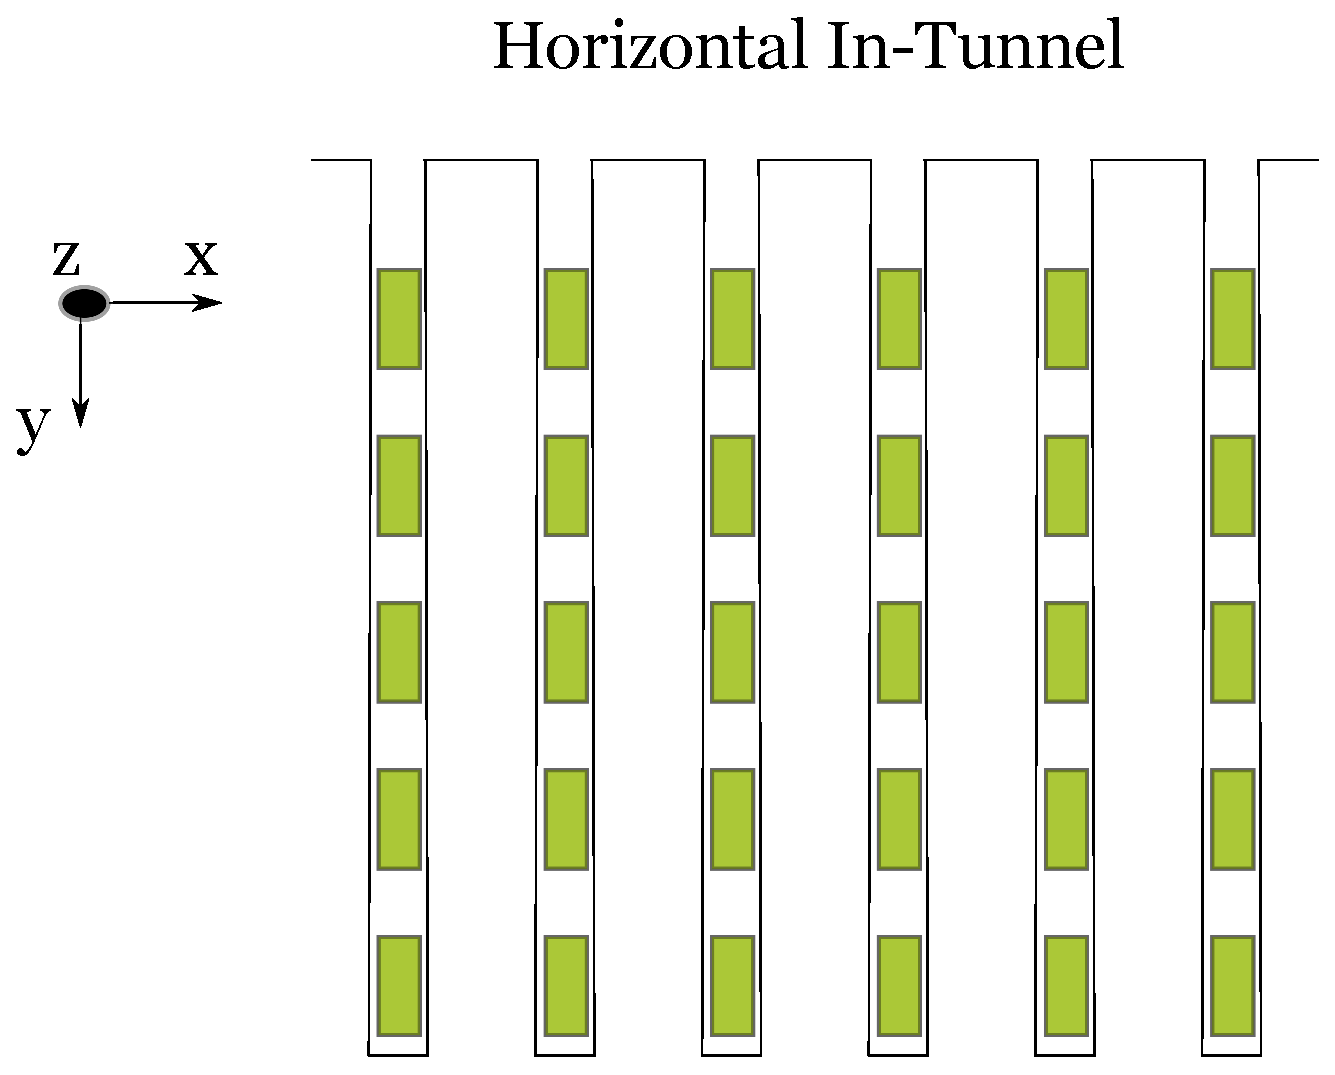
\includegraphics[width=0.8\textwidth]{horizontal.eps}
    \end{figure}
    \begin{figure}[h!]
      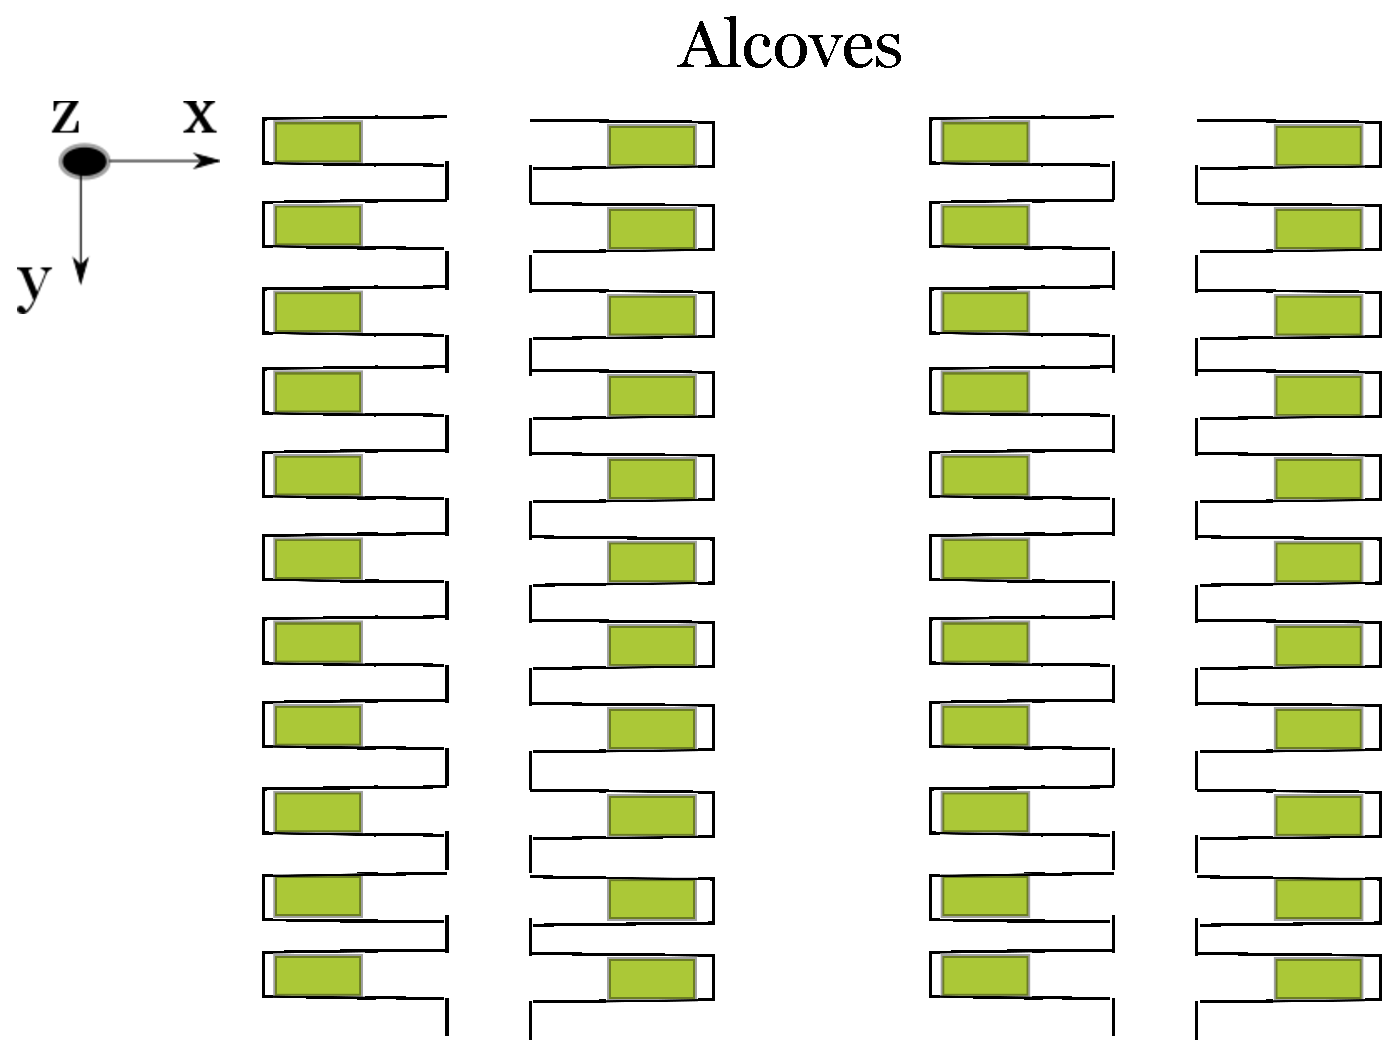
\includegraphics[width=0.8\textwidth]{alcoves.eps}
    \end{figure}
  \end{minipage}
\end{frame}

\begin{frame}[ctb!]
  \frametitle{All Disposal Environments}
  % Table
  %        File: geos_tab.tex
%     Created: Thu Aug 04 11:00 AM 2011 C
% Last Change: Thu Aug 04 11:00 AM 2011 C
%
\begin{table}[h!]
  \centering
  \footnotesize{
  \begin{tabular}{|l|r|r|r|r|}
    \multicolumn{5}{c}{\textbf{Features of Various Concepts}}\\
    \hline
    Feature & Clay & Granite & Salt & Deep Borehole \\ 
    \hline
    \multicolumn{5}{|c|}{\textbf{Hydrology}}\\
    \hline
    Total Porosity $[\%]$    & 34-60  & 0.1 & 0.5 & 0-0.5 \\ 
    Eff. Porosity $[\%]$ & 0.5-5 & 0.0005 & 0.1 & 0.00005-0.01 \\ 
    Conductivity$[m/s]$ & $10^{-11} - 10^{-9}$ & 
    $10^{-6}-10^{-5}$ & $10^{-12}-10^{-10}$ & 
    $10^{-13}-10^{-4}$ \\ 
    Fracturation & none & high & none & low at depth \\ 
    \hline
    \hline
    \multicolumn{5}{|c|}{\textbf{Geochemistry}}\\
    \hline
    Reducing & Near \& Far Field & NF only  & NF only & NF only \\
    Oxidizing & none & Slight in FF & Slight in FF & Slight in FF \\
    Salinity & higher at depth & higher at depth & high & high \\
    pH & $\sim7$ & $\ge7$ & $\ge7$ & $\sim7$ \\
    \hline
    \hline
    \multicolumn{5}{|c|}{\textbf{Design}}\\
    \hline
    Waste Package & Steel, Cu & Steel, Cu & Steel & Steel,Cement \\
    Buffer & -,Fo-Ca,Cement & Fo-Ca,Cement & Crushed Salt & -,Fo-Ca,Cement\\ 
    Depth & 100-500 m & 100-500 m & 100-500m & 3-5km \\ 
    Emplacement & Vert.,Horiz,Alcove & Vert.,Horiz. & Alcove & Vert. \\ 
    Packages/Gallery & one, many & one, many & one, two & 400 \\ 
    \hline
    \hline
    \multicolumn{5}{|c|}{\textbf{Thermal Behavior}}\\
    \hline
    Buffer Limit $[^{\circ}C]$ & 100 (Fo-Ca) & 100 (Fo-Ca) & 180 & 100 (Fo-Ca) \\ 
    Host Limit $[^{\circ}C]$   & 100 (alteration)  & 200 (cracking) & 180 (brines) & none \\ 
    Conductivity $[\frac{W}{m{\cdot}K}]$ & $1-2$ & $2-4$ & $\sim4$  & $2-4$ \\ 
    Coalesence & yes & no & yes & no \\ 
    \hline
  \end{tabular}
  }
  \label{tab:geos_tab}
\end{table}
%  \cite{stober_hydraulic_2006} 

\end{frame}

